\chapter{Experimental measurement system and procedures}
\label{chap.experimental}

\section{Overview}

Thus far we have considered flux noise in SQUIDs and qubits in a theoretical context. However, the bulk of our work is concerned with the experimental characterization of flux noise in SQUIDs. The success of this endeavor relies on a robust experimental measurement system that satisfies a number of stringent requirements. First and foremost, because we seek to accurately measure the intrinsic noise in SQUIDs, which are themselves ultra-low-noise devices, every care must be taken to insure that the measurement system produces as little noise as possible. In this same thread, $1/f$-noise measurements at low frequencies are necessarily slow measurements, which entails that the system must be ultra-stable over time scales on the order of hours. As noise originating from myriad sources---electronic and mechanical as well as temperature and magnetic field fluctuations, for example---can couple into the measurement, the design considerations are considerable.

We also seek to characterize the flux noise as a function of device temperature, which means that we need a refrigeration apparatus that can hold a stable temperature from approximately 0.1~K up to 4~K. Standard dilution refrigerators are quite capable of reaching such temperatures, but we shall see that care is needed to achieve the required stabilities well in excess of 1 part in $10^4$.

For a number of reasons, it is advantageous for the system to have the ability to cool multiple SQUIDs in a single cool-down and to measure each one individually. On one hand, the length of the cool-down and warm-up procedures of our dilution refrigerator means that considerable time is saved over cooling each SQUID individually. On another hand, cooling several SQUIDs simultaneously eliminates many potential confounding factors---trapped magnetic fields, for example---that could conceivably cause differences between measurements from different cool-downs.

In this Chapter we review the experimental design and implementation as well as the validation, calibration, and measurement procedure. The main components of the system are the [@@@ probably put the sections here], which we now discuss in detail.

\section{Measurement overview}

\begin{figure}
\centering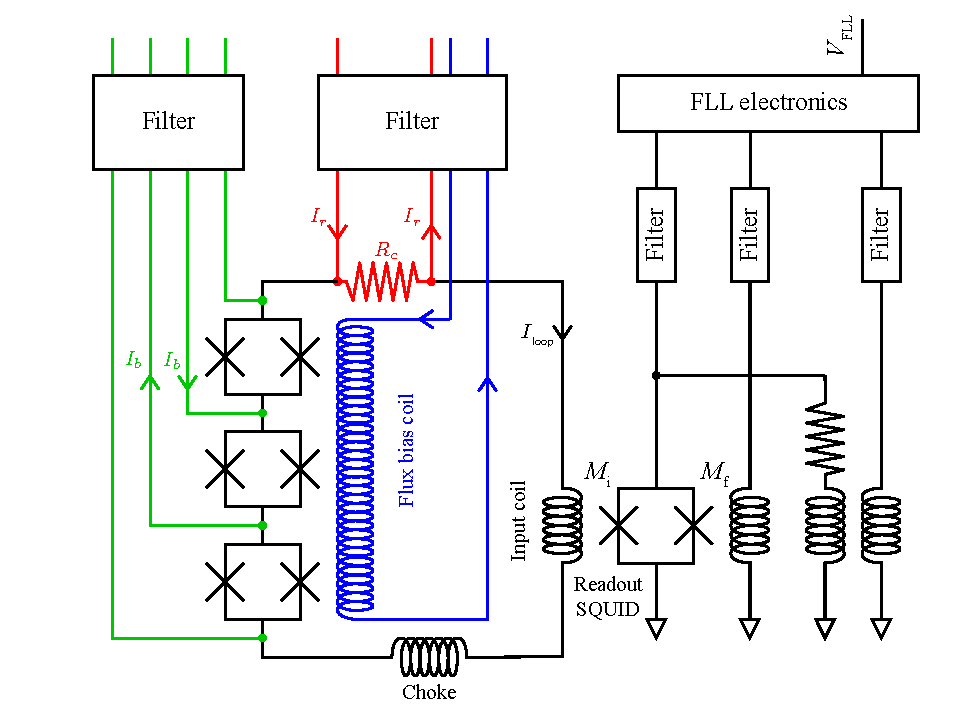
\includegraphics{experimental/Fig_schematic}\\
\caption[Schematic of measurement system]{Configuration of measurement system to measure flux noise in three SQUIDs. The bias current $I_b$ shown enables the measurement of the middle SQUID. The static voltage across the SQUID is canceled by the current $I_r$ applied to the compensating resistor $R_c$. [@@@ transformer ratios]}
\label{fig:experimental:schematic}
\end{figure}

The principle behind our measurement technique is that a SQUID biased into the normal state generates fluctuations based on changes in its critical current and the flux through its loop. Naturally, these fluctuations are quite small and cannot be read directly using even the best room-temperature amplifier. Therefore, we use a second SQUID, operated in a standard flux-locked loop (FLL) configuration, to detect the fluctuations. The fluctuations of the measured SQUID are monitored for long periods of time, converted to spectral densities, and subsequently analyzed.

The basis of our system is the circuit schematic illustrated in Fig.~\ref{fig:experimental:schematic}, where we have modified the design used by Wellstood~\citep{Wellstood:thesis} in order to accommodate multiple measured SQUIDs. In the circuit, several SQUIDs are connected in series with a small compensating resistor $R_c$, the input coil to the readout SQUID, and a choke inductor, which prevents high-frequency cross-talk between SQUIDs. Appropriate wiring to the circuit allows us to inject currents across the compensating resistor and each of the SQUIDs. To make a measurement, we begin by injecting a current $I_b$ through a particular SQUID and increasing it until the SQUID enters the normal state with voltage $V_{\text{SQUID}}$. At this point, most of the current bias passes through the measured SQUID, but a small amount $\Vsquid/R_c$ is shunted through the compensating resistor. If $I_b$ is increased further, a fraction $R_c/(R_d+R_c)$ of the current passes through the compensating resistor, where $R_d$ is the dynamic resistance of the measured SQUID. For reasons we discuss later, $R_c \ll R_d$ by design. If large enough, the shunted current that flows around the big loop can drive the other SQUIDs normal, where they begin to add their own intrinsic noise. To prevent this, a current $I_r$ is passed through the compensating resistor until $V_{\text{SQUID}} = I_r R_c$ and no net current flows around the loop, ensuring that the SQUIDs not under measurement remain superconducting and contribute no noise.

At this point, a variation in the critical current of the SQUID will redistribute the bias currents to the circuit. For instance, if the critical current suddenly drops, a fraction of $I_b$ will be diverted around the big loop, through $R_c$ and the input coil, thereby introducing a flux offset in the readout SQUID. The FLL, which is operated above 100~kHz, rapidly cancels this offset by increasing the current to a feedback coil (Fig.~\ref{fig:experimental:schematic}) until the flux offset is canceled. A voltage $\Vfll$ proportional to the feedback current and, correspondingly, the current circulating the loop is read at the output of the FLL. For small variations in the measured SQUID, the response is linear so that $\Vfll$ is also proportional to both the critical current of the SQUID. We now discuss the conversion factors as well as our choice of circuit and device parameters, chosen to optimize the sensitivity to the fluctuations.

Operated in this configuration, any single measurement is insufficient to discern the origin of the fluctuations that we measure. The noise we measure could originate from intrinsic critical current noise within the junctions; flux noise in the SQUID, which, in turn, modulates the critical current of the SQUID; or noise in the measurement or bias circuitry. Therefore, to verify our SQUID noise measurements, we must first verify that the noise of our bias and readout circuitry is negligible. Next, in order to distinguish between critical current and flux noise, we utilize the property of the SQUID whereby its sensitivity to flux ($\partial I_c/\partial\Phi$) varies as a function of its flux bias [@@@ ref in Chap 1]. By varying the flux bias and corresponding sensitivity of the SQUID, we can verify that the noise from the various spectra scales as an effective flux.

\subsection{Optimal circuit and device parameters}

\begin{figure}
\centering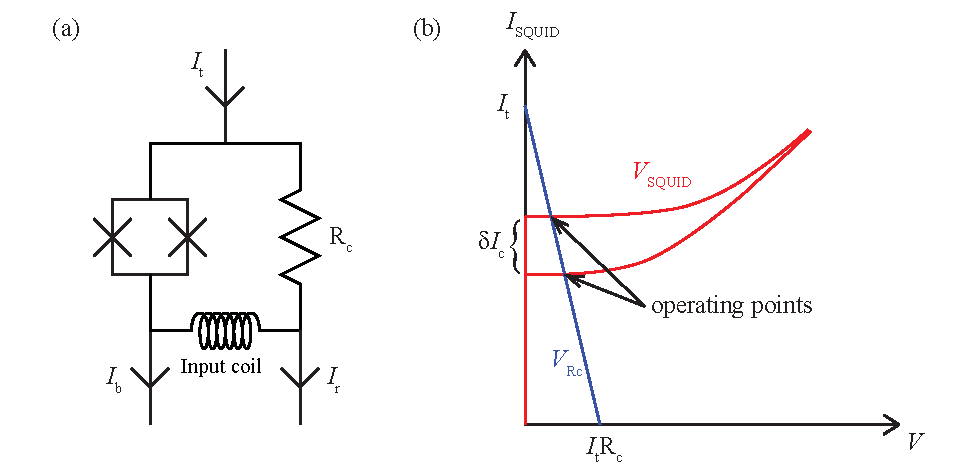
\includegraphics{experimental/Fig_loadline}\\
\caption[Bias and operating points of measured SQUID]{Bias and operating points of measured SQUID. (a) Simplified schematic of the typical biasing of a measured SQUID. (b) Current-voltage characteristics of a SQUID (red) for a small change in critical current. The load line for $R_c$ (blue) is calculated as follows. For zero current flowing through $R_c$, $V_{R_c} = 0$ and the current through the SQUID, $I_{\text{SQUID}}$, is maximum: $I_{\text{SQUID}} = I_t$. For $I_{\text{SQUID}} = 0$, the total current flows through $R_c$ and $V_{R_c} = I_t R_c$. The equilibrium solution occurs when $V_{\text{SQUID}} = V_{R_c}$, which is the intersection of the two curves. Therefore, $\delta I_c$ causes the operating points to change little in voltage, but maximally in current.}
\label{fig:experimental:loadline}
\end{figure}

% Optimization of Rc
In general, we choose parameters to maximize the change in $\Vfll$ for a given change in critical current or flux in the measured SQUID. First, we discuss the value of the compensating resistor. In Fig.~\ref{fig:experimental:loadline}(a) we show a simplified schematic of the typical biasing of a SQUID, omitting the superconducting SQUIDs; here, $I_t = I_r + I_b$ is the total current applied to the circuit. Ultimately, we seek to maximize the change in current through the input coil for a given change in SQUID critical current, $I_c$. In this familiar circuit, we recognize that if $R_c \gg R_d$, the SQUID is effectively current biased. That is, if the critical current of the SQUID decreases slightly, $V_{\text{SQUID}}$ will increase by $\delta V$ and the current through $R_c$ will increase by only $\delta V/R_c$, which, by construct, is very small. However, if $R_c \ll R_d$, the SQUID is effectively voltage biased. We show this situation in Fig.~\ref{fig:experimental:loadline}(b), using the concept of load lines because the SQUID is a nonlinear circuit element. In this scenario, a decrease $\Delta I_c$ in the $I_c$ of the SQUID corresponds to a maximum increase in increase of current through $R_c$ and, correspondingly, the input coil of the readout SQUID $\Delta I_{\text{loop}}$,
\begin{align}\label{Eqn:dIloop_dIc}
\Delta I_{\text{loop}} = \frac{1}{1+R_c/R_d} \Delta I_c.
\end{align}
For typical values of $R_d \sim 10~\Omega$, $R_c$ should be on the order of $1~\Omega$. From Eq.~\eqref{Eqn:dIloop_dIc}, we see that values of $R_c$ much less than $R_d/10$ do not offer much additional signal and can, in fact, degrade the performance of the system if $R_c$ is too low. We also see that for $R_c \ll R_d$, $\Delta I_{\text{loop}} \approx \Delta I_c$ and throughout this thesis we will often use $\Delta I_{\text{loop}}$ and $\Delta I_c$ interchangeably.

% FLL and readout SQUID parameters
With a small value of $R_c$, we ensure that fluctuations in the readout SQUID generate maximum current fluctuations through the input coil of the readout SQUID. In turn, we maximize the flux coupled into the readout SQUID by using the largest feasible mutual inductance for the input coil $M_i$. In general, $M_i \sim 10~\text{nH}$, or $M_i^{-1} \sim 0.1~\mu\text{A}/\Phi_0$. Conversely, we aim to make the mutual inductance of the feedback coil $M_f$ small ($\sim 0.5~$nH) so that the feedback current is relatively large. Finally, the feedback resistor $R_{\text{feedback}}$, which sets the conversion factor between the feedback current and $\Vfll$, is chosen to be large ($\gtrsim 100~\text{k}\Omega$). Thus, $\Vfll$ is related to $I_{\text{loop}}$ via
\begin{align}\label{fig:experimental:Vfll_Iloop}
\Vfll = R_{\text{feedback}} \left( \frac{M_i}{M_f} \right) I_{\text{loop}},
\end{align}
and the FLL has a transconductance on the order of $10^6$~V/A.

% Optimization of junction parameters
It is also possible to optimize the junction parameters of the SQUIDs. By varying the value of the shunt resistance $R$ and critical current of the junctions, we can modify the level of white noise and flux sensitivity, respectively. At high enough frequencies---typically, above 10 to 100~Hz when the SQUID is biased at maximum flux sensitivity---the white noise generated by the shunt resistors dominates both the flux and critical current noise of the SQUID. As a current, the white noise magnitude scales as $R^{-1}$~\citep{Likharev:1972} [@@@ cover in Chap 1], which indicates that we can reduce the white noise level by increasing $R$. Because $\partial I_c/\partial\Phi$ is roughly proportional to $I_c$ [@@@ cover in Chap 1], we can also increase the sensitivity of our measurement to flux in the measured SQUID. These two criteria suggest that one should increase $R$ and $I_c$ as much as possible in order to maximize the relative current variations due to flux noise. However, our measurements require that the SQUIDs operate non-hysteretically, that is, $\beta_c = 2\pi I_0 R^2 C/\Phi_0 < 1$~\citep{Stewart:1968,McCumber:1968}, so that $R$ and $I_0$ cannot both be increased without bound. Here, $I_0 = I_c/2$ and $C$ are the average junction critical current and capacitance, respectively. For fixed critical current density $j_c$ and constant capacitance per unit area $C/A$, $I_0$ is typically varied by changing the junction area $A$ so that $I_cR^2 C \propto A^2 R^2$. Assuming that one designs a SQUID for fixed $\beta_c < 1$, this constraint also implies a fixed product $I_c R$. Because the white noise decreases only as $R^{-1}$ but the flux sensitivity increases as $(\partial I_c/\partial\Phi)^2 \propto I_c^2$, we see that it is most advantageous to increase $I_c$ as much as possible, even at the cost of decreasing $R$.

\section{Implementation}

\begin{figure}
\centering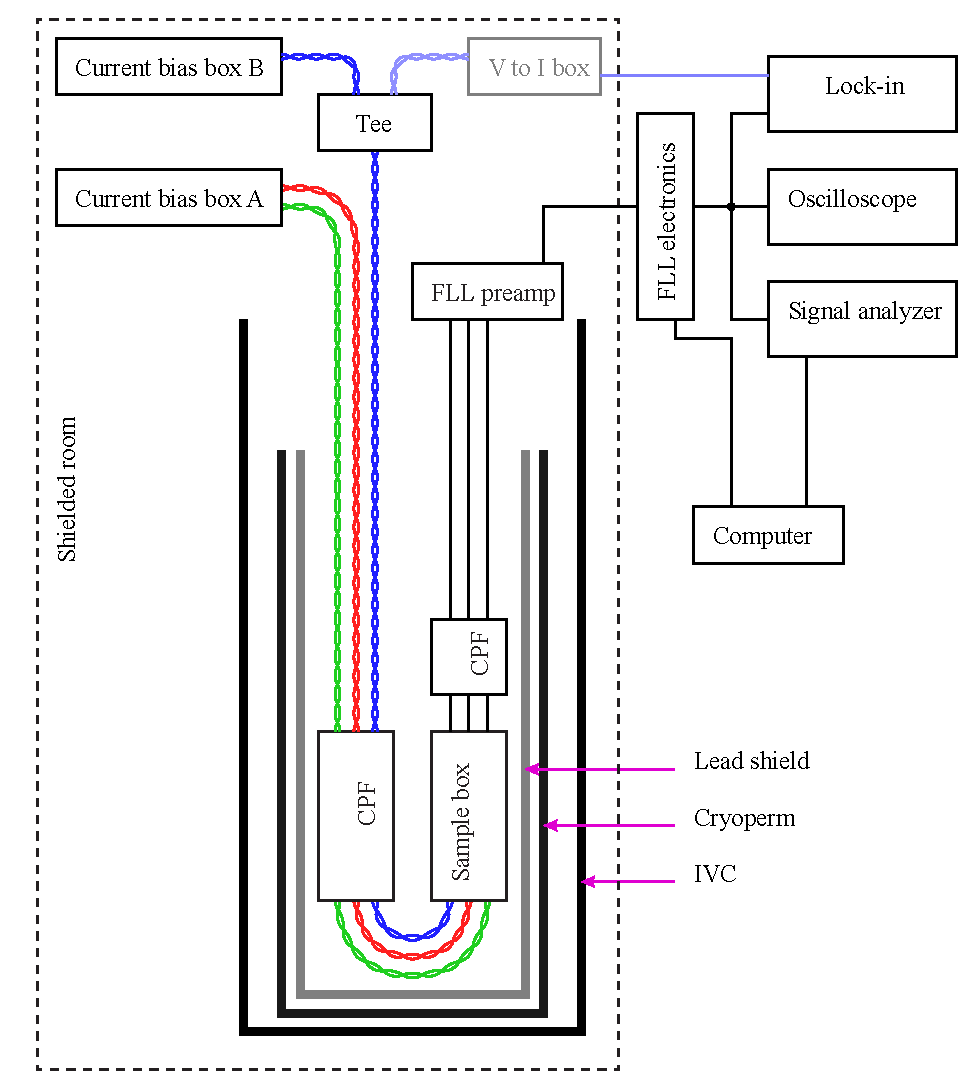
\includegraphics{experimental/Fig_meas_schematic}\\
\caption[Schematic of measurement system]{Schematic of measurement system. The sample is mounted to the cold finger of a dilution refrigerator and is surrounded by a combination shield of Pb and Cryoperm for magnetic shielding. All lines are low-pass filtered using copper powder filters (CPF) and discrete filters. The typical configuration of bias boxes and readout equipment is shown. The shaded portion is connected only when measuring $\partial I/\partial \Phi$, not when acquiring noise data. [@@@ This fig probably runs over the bottom margin! @@@ Add discrete filters]}\label{Fig:meas_schem}
\end{figure}

We now discuss the specifics of how we implement the measurement system, which is shown schematically in Fig.~\ref{Fig:meas_schem}. The SQUIDs to be measured, which are typically fabricated onto a single chip, are first mounted and wire-bonded onto a circuit board in one of the chambers of a copper sample box (Fig.~\ref{fig:experimental:sample_box}). Flux bias is provided via either an on-chip coil or a coil mounted in the circuit board, directly below the chip. The compensating resistor, which is simply a short segment of resistance wire, is also mounted to the circuit board. The readout SQUID is located in another chamber on the opposite side of the box in order to prevent cross-talk between SQUIDs. Intermediate chambers contain the choke inductor and a cold transformer on the voltage line of the readout SQUID, which is used both to step up the voltage and to impedance match to the room-temperature amplifier. Once the sample is mounted into the box, a Cu lipped lid is attached. For magnetic shielding, the inner surfaces of both the box and lid are electroplated with approximately $200~\mu$m of Pb.

\begin{figure}
\centering\includegraphics[width=6.5in]{experimental/sample_box.jpg}\\
\caption[Photo of sample box]{Photo of sample box. Six chambers separate the various portions of the measurement circuit. The circuit board holding the measured SQUIDs is on the left. On the right is the board holding the readout SQUID. The chambers in the middle hold the choke inductor and cold transformer, wound around molypermalloy powder (MPP) cores, which work well at cryogenic temperatures.}
\label{fig:experimental:sample_box}
\end{figure}

\begin{figure}
\centering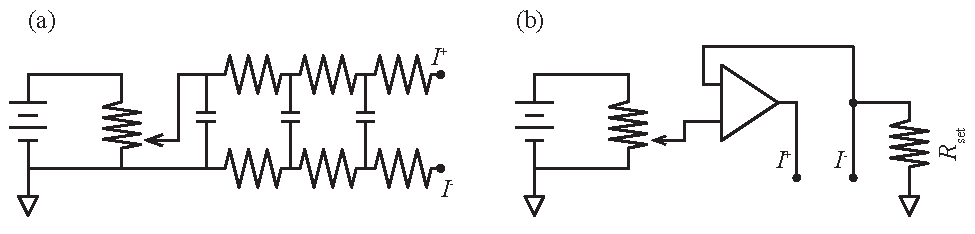
\includegraphics{experimental/Fig_current_supplies}\\
\caption[Circuit schematics of current supply boxes]{Circuit schematics of current supply boxes. (a) ``Passive'' circuit design, type A. Li-ion battery sources a current controlled by a 10-turn potentiometer. This design is useful for sourcing $\lesssim 100~\mu$A. (b) ``Active'' circuit design, type B. The Li-ion battery and 10-turn potentiometer provide a stable voltage source input to the op-amp (ISL28134). $R_{\text{set}}$ sets the current output range, which, for this op-amp, is approximately $60~\mu$A. Since the op-amp sources the current, the discharge on the Li-ion batter is minimal.}
\label{fig:experimental:bias_boxes}
\end{figure}

The sample box is then mounted onto the cold finger of an Oxford DR200 dilution refrigerator. In addition to the Pb plating of the sample box, further attenuation and shielding of external magnetic fields are provided by two concentric cans of Pb and Cryoperm. Electrical signals are carried via three 4-conductor Reichenbach cables for the various biasing of the measured SQUIDs and three SMA coaxial cables for the current bias, voltage readout, and flux feedback current of the readout SQUID. All lines are rf-filtered using standard copper powder filters (CPFs) and low-pass filtered using discrete filters. Bias currents are provided via lithium-ion battery-powered boxes using one of two circuit designs, shown in Fig.~\ref{fig:experimental:bias_boxes}. The current biases for $I_b$ and $I_r$ typically need to source only tens of microamps and use the ``passive'' design  [Fig.~\ref{fig:experimental:bias_boxes}(a)]. The current bias for the flux bias of the measured SQUIDs, however, can require in excess of 10~mA, so we use an ``active'' source [Fig.~\ref{fig:experimental:bias_boxes}(a)]. Both designs rely on the extremely flat discharge voltage of Li-ion batteries, which allows us to use them as simple, yet stable, voltage references. For the readout and control electronics of the FLL, we have used two different commercial packages available from Easy SQUID and STAR Cryoelectronics, respectively. Both packages come with amplification units, which we attach directly atop the fridge. For additional isolation and electric shielding, the fridge and the electronics mentioned thus far are located within a shielded room, consisting of an electrically continuous copper sheet (Fig.~\ref{Fig:meas_schem}).

The FLL preamplification box interfaces with the control electronics, external to the shielded room, via a filtered DB9 cable. The FLL control electronics in turn output $\Vfll$ and also connect to a computer, which provides control over the FLL parameters. The output $\Vfll$ is passed to a oscilloscope, which is used during the biasing procedure, and to an Agilent~35670A signal analyzer. It is also passed to a lock-in amplifier, which is used to measure $\partial I/\partial \Phi$, which is described in Section~\ref{chap:exp:sec:meas_proc}.

Data are acquired using the signal analyzer and sent to a computer for analysis and storage. Under normal operation, the signal analyzer acquires data and computes the spectral density, which is stored in a buffer that the computer can access. However, we have found that it is much more advantageous to use the signal analyzer to capture the raw time series of $\Vfll$. A single time capture allows us to compute multiple FFT's with differing numbers of averages to form a single, stitched spectrum. [Appendix on how this is done?] In a typical measurement, the sampling rate and length of time capture, which defines the buffer size, are programmed into the signal analyzer via the computer interface and a custom LabVIEW program (Signal Analyzer Controls in Fig.~\ref{fig:experimental:LabVIEW_time_capture}). The signal analyzer then fills the buffer and uploads the time series to the LabVIEW program, where we can save it to disk, together with a header file with details of the measurement, and compute the spectral density. For more advanced plotting and analysis functions, we use a suite of Matlab programs that we have written for this purpose.

\begin{figure}
\centering\includegraphics[width=6.5in]{experimental/LabVIEW_time_capture.png}\\
\caption[Screenshot of LabVIEW time capture acquisition program]{Screenshot of LabVIEW time capture acquisition program. For a typical measurement, `Signal Analyzer Controls' set the sampling frequency and buffer size of the signal analyzer. `Run Time Capture' instructs the signal analyzer to start filling the buffer. Once the time capture finishes and is downloaded, we can compute the FFT in LabVIEW with parameters set in `LabVIEW FFT Controls'. A `Notes' section allows the user to specify details of the measurement; these notes, along with the parameters of `Signal Analyzer Controls' are saved to the specified file and path. Several different time captures can be queued to run sequentially. [@@@ Need to take better capture and add FFT.]}
\label{fig:experimental:LabVIEW_time_capture}
\end{figure}

[@@@ anything else?]

%\begin{figure}
%\centering\includegraphics[height=4in]{experimental/fridge.jpg}\\
%\caption{Picture of fridge}
%\label{fig:experimental:fridge_photo}
%\end{figure}

\section{Calibration and validation}

To validate the system, we must first measure certain parameters in order to calibrate conversion factors and then verify that the readout and bias electronics are sufficiently low-noise. First, we seek to calibrate the output of the FLL; that is, we want to know $\partial\Iloop/\partial\Vfll$. From Eq.~\eqref{fig:experimental:Vfll_Iloop}, this means we need to measure $M_i$, $M_f$, and $R_{\text{feedback}}$. There is a trick, however, that allows a direct calibration of $\partial\Vfll/\partial\Phi_a$, where $\Phi_a$ is the flux in the readout SQUID. Then,
\begin{align}\label{Eqn:dIloop_dVfll}
\frac{\partial\Iloop}{\partial\Vfll} = \left(\frac{\partial\Iloop}{\partial\Phi_a}\right) \left(\frac{\partial\Phi_a}{\partial\Vfll}\right) %
= M_i^{-1} \left(\frac{\partial\Vfll}{\partial\Phi_a}\right)^{-1}.
\end{align}
To measure $\partial\Vfll/\partial\Phi_a$, we begin by locking the FLL with zero current in the big loop and we record the $\Vfll$. Next, we unlock the FLL, inject a current into the input coil corresponding to approximately one flux quantum, and lock the loop. We can do this even with the SQUIDs bonded into the loop by injecting a current $I_r$ across the compensating resistor. Since the SQUIDs are superconducting, the current will flow through the lowest resistance path; that is, all the current will flow through the SQUIDs and input coil. With the loop locked, we now reduce the bias current back to zero and again record $\Vfll$. The difference in recorded voltages $\Delta \Vfll$ corresponds to one $\Phi_0$ in the readout SQUID, $\partial\Vfll/\partial\Phi_a = \Delta \Vfll / \Phi_0$, which is about 0.5~V/$\Phi_0$ for our system. This method is described in detail in Sec.~2.10a of Ref.~\citep{Wellstood:thesis}. The mutual inductance of the input coil $M_i$ can be readily measured by injecting a known bias current into the circuit---again, across the compensating resistor if SQUIDs are in the circuit---and measuring the response in $\Vfll$. For $M_i \approx 10$~nH as in our system, $\partial\Iloop/\partial\Vfll \approx 0.4~\mu$A/V.

Next, we must calibrate $\Vfll$ to changes in the measured SQUID. Changes in $I_c$ are related to $\Vfll$ via
\begin{align}\label{fig:experimental:dIc_dVfll}
\frac{\partial I_c}{\partial\Vfll} = \left(\frac{\partial I_c}{\partial\Iloop}\right) \left(\frac{\partial\Iloop}{\partial\Vfll}\right) %
\approx \frac{\partial\Iloop}{\partial\Vfll}
\end{align}
by Eq.~\eqref{Eqn:dIloop_dIc} for $R_c \ll R_d$. For our applications, Eq.~\eqref{fig:experimental:dIc_dVfll} is sufficiently accurate---10\% for $R_c = R_d/10$---as we are not focused on highly accurate measurements of critical current noise.

To scale $\Vfll$ to an equivalent flux noise, we seek to measure the change $\Delta\Vfll$ in response to a known applied flux in the measured SQUID $\Delta\Phi_m$. In order to do so, we must first measure the mutual inductance $M_m$ between the flux bias coil (which is either fabricated on-chip or mounted in the circuit board to which the chip is mounted) and the measured SQUID. We readily accomplish this by injecting a known current $I_\Phi$ into the coil and monitoring the response of the SQUID, which is periodic in flux. For example, the difference in flux, achieved by a difference in current $\Delta I_\Phi$ in the coil, that separates maxima in SQUID critical current is $1~\Phi_0$. Therefore, the mutual inductance is simply $M_m = \Phi_0/\Delta I_\Phi$. In principle, only one period is sufficient for this measurement, but we typically measure over five or more and perform a linear regression for better accuracy. In addition, we have found that measuring the flux bias corresponding to a minimum SQUID critical current, rather than a maximum, is more precise because the $I_c$--$\Phi$ characteristics are much sharper at $(n+\tfrac{1}{2})\Phi_0$ than at $n\Phi_0$. Finally, to measure $\partial\Vfll/\partial\Phi_m$ we inject a known current, converted to a flux in the measured SQUID via $M_m$, and measure the response in $\Vfll$. This calibration, which must be performed before each flux noise measurement, is described in greater detail in the next Section.

After establishing the relevant conversion factors, we want to characterize the noise of the measurement system. With the measured SQUIDs in the superconducting state, the major sources of noise are (i) the amplification and readout electronics of the FLL, (ii) the intrinsic critical current and flux noise of the readout SQUID, and (iii) the Nyquist noise of the compensating resistor~\citep{Nyquist:PR:1928}. While it is possible to measure the noise from (i) and (ii) independently, the characterization process is complicated, lengthy, and involves several cooldowns to 4~K. A much simpler method exists that puts an upper bound on the combined noise of (i) and (ii). With accurate knowledge of the compensating resistance $R_c$ and temperature $T$, we can calculate the Nyquist current noise spectral density as $S_{I,R_c} = 4 k_B T/R_c$. By comparing the measured to predicted noise, we can estimate the noise added by the readout. In addition, we can confirm the calibration of the system. We find that our electronics add approximately $3~(\text{pA})^2$/Hz of white noise, which is negligible compared to $S_{I,R_c}$ for $T \gtrsim 0.3$~K and $R_c \approx 0.5~\Omega$. Above this temperature, agreement between measurement and prediction is better than 10\%. This measurement also yields the $1/f$ noise of (i) and (ii); (iii) contributes no $1/f$ noise. We found that the Easy SQUID readout system exhibited significantly more $1/f$ noise than the Cryoelectronics, which was a problem when measuring low-noise SQUIDs.

Finally, we remark that [temperature noise, explained in detail in Appendix?]

\section{Measurement procedure}\label{chap:exp:sec:meas_proc}

[The following section probably needs a bit more detail.]

The SQUID is variably sensitive to small changes in flux depending on its flux bias, ranging from zero sensitivity when biased at $n\Phi_0$ to maximum sensitivity at nominally $(n\pm\tfrac{1}{4})\Phi_0$. To measure flux noise, clearly we must bias the SQUID at a point where it is sensitive to changes in flux. However, as discussed in Chapter~\ref{chap:intro}, the total noise generated by the SQUID includes both critical current and flux noise. Furthermore, the magnitude of the contribution of asymmetric critical current variations varies as the flux sensitivity. Therefore, if the critical current noise is significant compared to the flux noise, its contribution is very difficult to subtract accurately from the total noise. If the critical current noise is much smaller than the flux noise, however, we can safely neglect its contribution. Therefore, we first characterize the critical current noise of the SQUID to ensure that it is negligible and then we measure at maximum flux sensitivity.

To measure the critical current noise of a SQUID we first bias it into the voltage state---typically $\Vsquid \sim 5~\mu$V---and null the induced loop current $\Iloop$ with an appropriate current through the compensating resistor. At this point, we vary the flux bias $\Phi_m$---adjusting the current bias $I_b$ as the critical current changes---to the point where $I_c$ is maximum and $\partial I_c/\partial \Phi_m = 0$, which corresponds to a flux bias of $n\Phi_0$. In this situation, a symmetric variation in the critical currents of the junctions will cause $I_c$ to vary, which, in turn, induces a current $\Iloop$ into the input coil of the readout SQUID as in Eq.~\eqref{Eqn:dIloop_dIc}. We acquire a time capture of $\Vfll$, sampled at approximately 1~kHz, for between 15~minutes to 1~hour, which is sufficiently long to characterize the noise at low frequencies (down to approximately $10^{-1}$~Hz to $10^{-2}$~Hz). From the time capture, we compute the spectral density, which we can scale to an equivalent current in the loop via Eq.~\eqref{Eqn:dIloop_dVfll}. At high frequencies, the spectrum is flat due to the white noise generated by the resistive shunts of the junctions. If the magnitude is large enough, the $1/f$ noise from symmetric critical current fluctuations will cause the observed spectral density to increase at low frequencies.

Once the critical current noise is characterized, we next seek to bias the SQUID at the point of maximum sensitivity to flux in order to measure its flux noise. In other words, we vary $\Phi_m$ until $\partial\Iloop/\partial\Phi_m$ is maximized. To measure $\partial\Iloop/\partial\Phi_m$, we first use the internal oscillator of a Stanford Research Systems SR830 lock-in amplifier and a custom voltage-to-current box to generate an oscillating current of known magnitude. As shown in Fig.~\ref{Fig:meas_schem}, the oscillating current is summed with the static flux bias current and injected into the flux bias coil of the measured SQUID. Using the measured value of $M_m$, we calculate the rms magnitude of oscillating flux $\Phi_{m,\text{osc}}$ applied to the measured SQUID. The oscillating flux causes $I_c$ and, correspondingly, $\Vfll$ to modulate. We use the lock-in to demodulate $\Vfll$ and compute the rms magnitude of the voltage oscillations $\Vfll{}_{\text{,osc}}$, from which we readily calculate
\begin{align}\label{Eqn:dIloop_dPhim}
\frac{\partial\Iloop}{\partial\Phi_m} = \frac{\Vfll{}_{\text{,osc}}}{\Phi_{m,\text{osc}}} %
\left(\frac{\partial\Iloop}{\partial\Vfll}\right).
\end{align}
To ensure that the response is linear, it is important that $\Phi_{m,\text{osc}} \ll \Phi_0$; in our measurements, $\Phi_{m,\text{osc}}/\Phi_0$ was typically between $10^{-2}$ and $10^{-3}$. Depending on the value of $\beta_L$, the flux bias corresponding to maximum $\partial\Iloop/\partial\Phi_m$ can vary from approximately $(n\pm\tfrac{1}{4})\Phi_0$ for SQUIDs with $\beta_L \approx 1$ to very near $(n\pm\tfrac{1}{2})\Phi_0$ for SQUIDs with $\beta_L \ll 1$~\citep{Tesche:JLTP:1977}. In spite of this detail, for brevity we will often refer to $\Phi_m = \tfrac{1}{4}\Phi_0$ as the bias corresponding to the maximum sensitivity.

With $\partial\Iloop/\partial\Phi_m$ maximized, we voltage bias the SQUID and null $\Iloop$ in the manner previously described, acquire a 1~hr time capture, and compute the spectral density. At this flux bias, $I_c$ is maximally sensitive to both asymmetric critical current and flux noise.
By comparing this spectrum to that acquired at $n\Phi_0$, we can readily determine the noise added by these two sources. We recall from our previous discussion in Sec.~\ref{Sec:sym_asym_Ic_noise} that $I_c$ variations due to asymmetric critical current variations are generally smaller than $I_c$ variations due to symmetric critical current variations: $S_{I_c,\text{asym}} \lesssim S_{I_c,\text{sym}}$. Therefore, a large difference in noise between the two spectra must be due to the flux noise. [@@@ Talk about Fig.~\ref{Fig:spectra_vs_bias}]

\begin{figure}
%\centering\includegraphics[width=6.5in]{experimental/LabVIEW_time_capture.png}\\
\caption[Blah]{Noise spectra versus bias.}
\label{Fig:spectra_vs_bias}
\end{figure}

As a further verification, we can verify that the observed noise increase scales as an equivalent flux. To do this, we reduce $\partial\Iloop/\partial\Phi_m$ to, say, half its maximum and again acquire data. If the observed noise is indeed due to flux variations, its magnitude referenced as a current in the input coil should scale as $(\partial\Iloop/\partial\Phi_m)^2$; that is, the spectral density at a particular frequency should be reduced by a factor of four compared to the spectrum acquired at $|\partial\Iloop/\partial\Phi_m|_\text{max}$. Of course, the white noise from the shunts, which dominates at high enough frequency, does not scale as a flux, so the ``knee'' between white current noise and $1/f$ flux noise will decrease in frequency, a fact that highlights the importance of acquiring data at maximum $\partial\Iloop/\partial\Phi_m$. [@@@ Reference Fig.~\ref{Fig:spectra_vs_flux_bias}]

\begin{figure}
%\centering\includegraphics[width=6.5in]{experimental/LabVIEW_time_capture.png}\\
\caption[Blah]{Proper scaling of flux noise. Noise spectra acquired at different values of $\partial\Iloop/\partial\Phi_m$.}
\label{Fig:spectra_vs_flux_bias}
\end{figure}

\section{Fits?}

After acquiring...

Appendix~\ref{App:stitch_spec}




\subsection{Lorentzian fits?}

\section{Low-frequency critical current noise}

[Make this an appendix instead?]








